
\section{Schwachstelle 5: Command-Shell zwischen spoon-Host und win.int.mb-reps.cool.datcom.prv} 
\label{sec:vuln5}
Über einen ungewöhnlichen SSH-Tunnel vom \texttt{spoon}-Host  zum \texttt{win.int.mb-reps.cool.datcom.prv}-Host, ist es möglich ohne Authentifizierung Zugriff auf den \texttt{win}-Host zu erlangen und beliebige Befehle mit den Rechten des \texttt{win}-Benutzers auszuführen.

\subsection{Wegbeschreibung der Schwachstelle}
\label{subsec:vuln5_way}
Weitere Analysen der Socket-Verbindungen auf dem \texttt{spoon}-Hosts haben ergeben, dass ein ungewöhnlicher und somit auffälliger Port 4444 vom \texttt{sshd}-Prozess (Prozess-ID: 1822) geöffnet wurde. Dabei ist dieser geöffnete Port nur für den localhost (IPv4 \& IPv6) verfügbar und kann somit nicht von anderen Netzwerkteilnehmern genutzt werden. Abbildung \ref{fig:vuln5_netstat} zeigt die Ausgabe des Befehls \texttt{netstat -tlpn}.

 \begin{figure}[htbp]
    \centering
    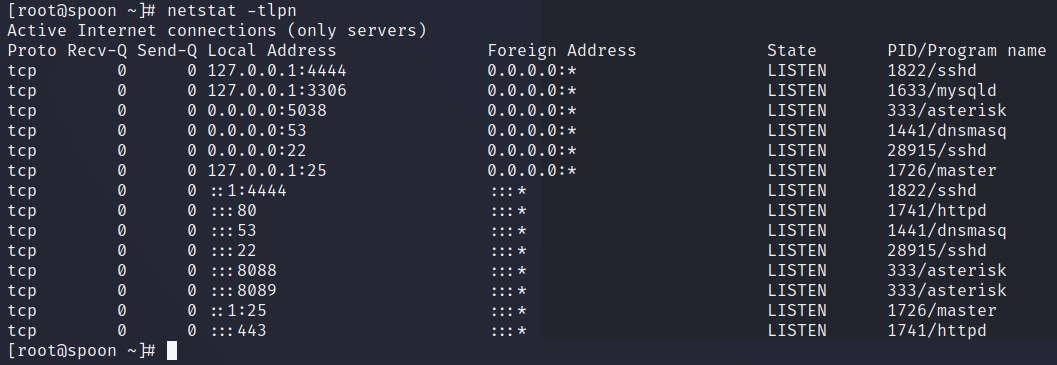
\includegraphics[width=\textwidth]{./img/vuln5_sshtunnel/spoon_netstat}
    \caption{Analyse der Socketverbindungen auf \texttt{spoon}.}
    \label{fig:vuln5_netstat}
\end{figure}

Mit dem Befehl \texttt{nc localhost 4444} und \texttt{python -c 'import pty; pty.spawn("/bin/bash")'} konnte anschließend eine Verbindung zum \texttt{win}-Host mit der IP-Adresse \texttt{172.16.34.42/24} und dem Benutzer \texttt{win (uid: 1000)} hergestellt werden (s. Abbildung \ref{fig:vuln5_spoon_nc_4444}). 

 \begin{figure}[htbp]
    \centering
    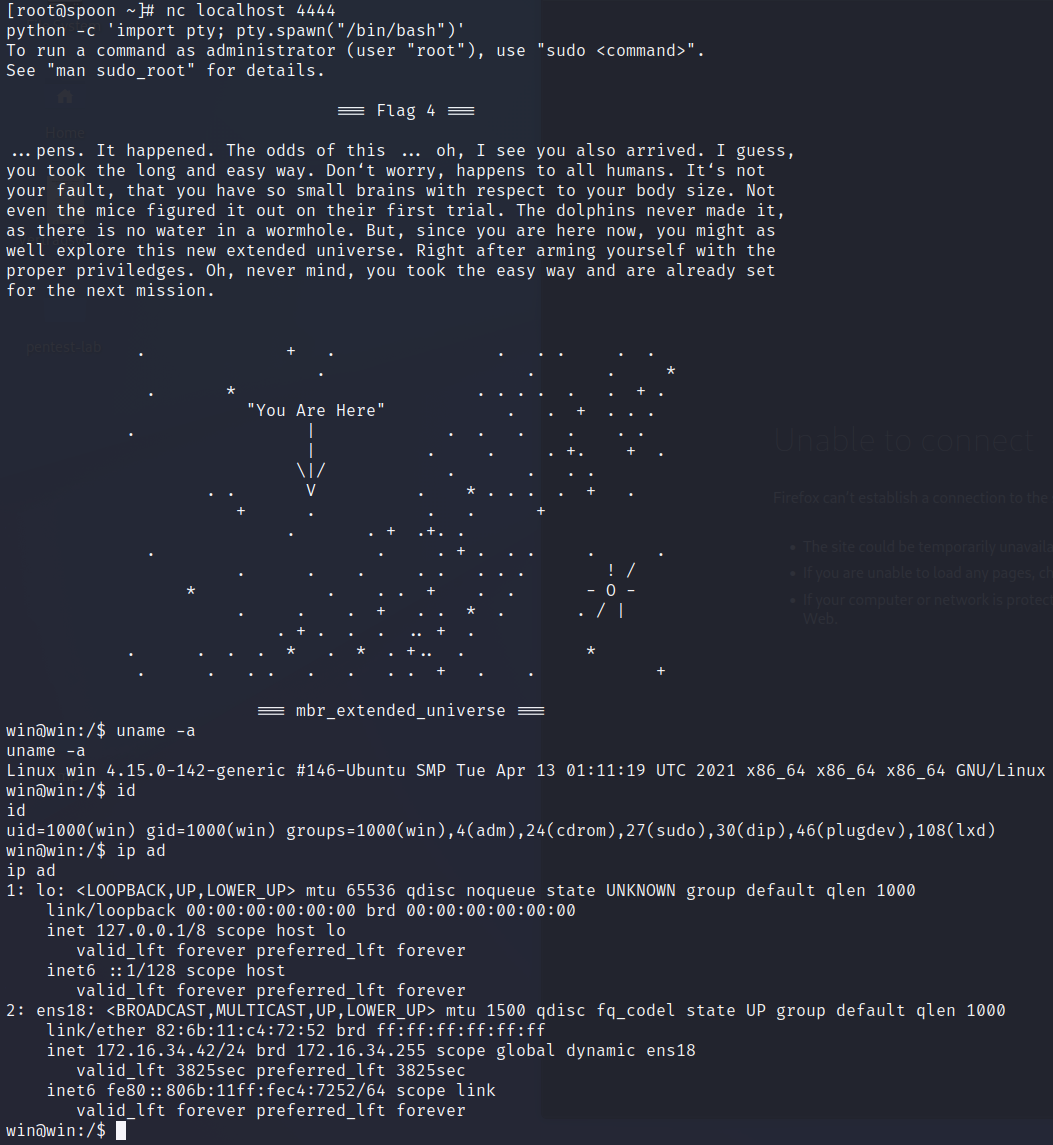
\includegraphics[width=\textwidth]{./img/vuln5_sshtunnel/spoon_nc_4444}
    \caption{Verbindung zum Host \texttt{win} herstellen.}
    \label{fig:vuln5_spoon_nc_4444}
\end{figure}

Da es sich ebenfalls um ein 64-bit Betriebssystem auf Basis von Ubuntu mit dem Linux-Kernel in der Version 4.15.0-142 handelt, kann auch in diesem Fall die Meterpreter-Payload von der Kali-Maschine heruntergeladen und gestartet werden (s. Abbildung \ref{fig:vuln5_spoon_meterpreter_start}).

 \begin{figure}[htbp]
    \centering
    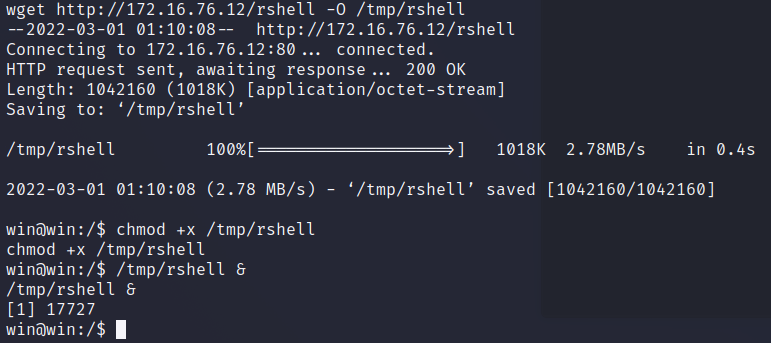
\includegraphics[width=\textwidth]{./img/vuln5_sshtunnel/win_meterpreter_start}
    \caption{Starten der Meterpreter-Payload auf dem \texttt{win}-Host.}
    \label{fig:vuln5_spoon_meterpreter_start}
\end{figure}

Von diesem Zeitpunkt an lassen sich beliebige Dateien des \texttt{win}-Systems extrahieren, weitere Dateien nachladen sowie Befehle mit den Berechtigungen des \texttt{win}-Benutzers ausführen.


\subsection{Risikobewertung}
Da die Socket-Verbindung vom Spoon-Host zum Win-Host nur über den auf Spoon lokal laufenden Port 4444 aufgebaut werden kann, aber für die Verbindung keine Authentifizierung benötigt wird, wird die Eintrittswahrscheinlichkeit mit MITTEL bewertet. Im Falle einer Kompromittierung über diesen Weg wird die Schadenshöhe aufgrund der limitierten Berechtigungen des \texttt{win}-Kontos mit MITTEL eingestuft.

Das Gesamtrisiko wurde daher mit \textcolor{orange}{MITTEL} bewertet.

\subsection{Empfohlene Gegenmaßnahmen}
Es wird empfohlen den Port 4444 und den dahinterliegenden SSH-Dienst zu beenden.

\subsection{Hinterlassene Spuren und Spurenbeseitigung}
Es wurde im \texttt{/tmp/}-Ordner die Reverse-Shell-Datei \texttt{rshell} hochgeladen, welche mit dem Befehl \texttt{rm /tmp/rshell} entfernt werden konnte.

